% This file was created by matlab2tikz.
%
%The latest updates can be retrieved from
%  http://www.mathworks.com/matlabcentral/fileexchange/22022-matlab2tikz-matlab2tikz
%where you can also make suggestions and rate matlab2tikz.
%
\definecolor{mycolor1}{rgb}{0.00000,0.44700,0.74100}%
\definecolor{mycolor2}{rgb}{0.85000,0.32500,0.09800}%
\definecolor{mycolor3}{rgb}{0.92900,0.69400,0.12500}%
\definecolor{mycolor4}{rgb}{0.49400,0.18400,0.55600}%
\definecolor{mycolor5}{rgb}{0.46600,0.67400,0.18800}%
%
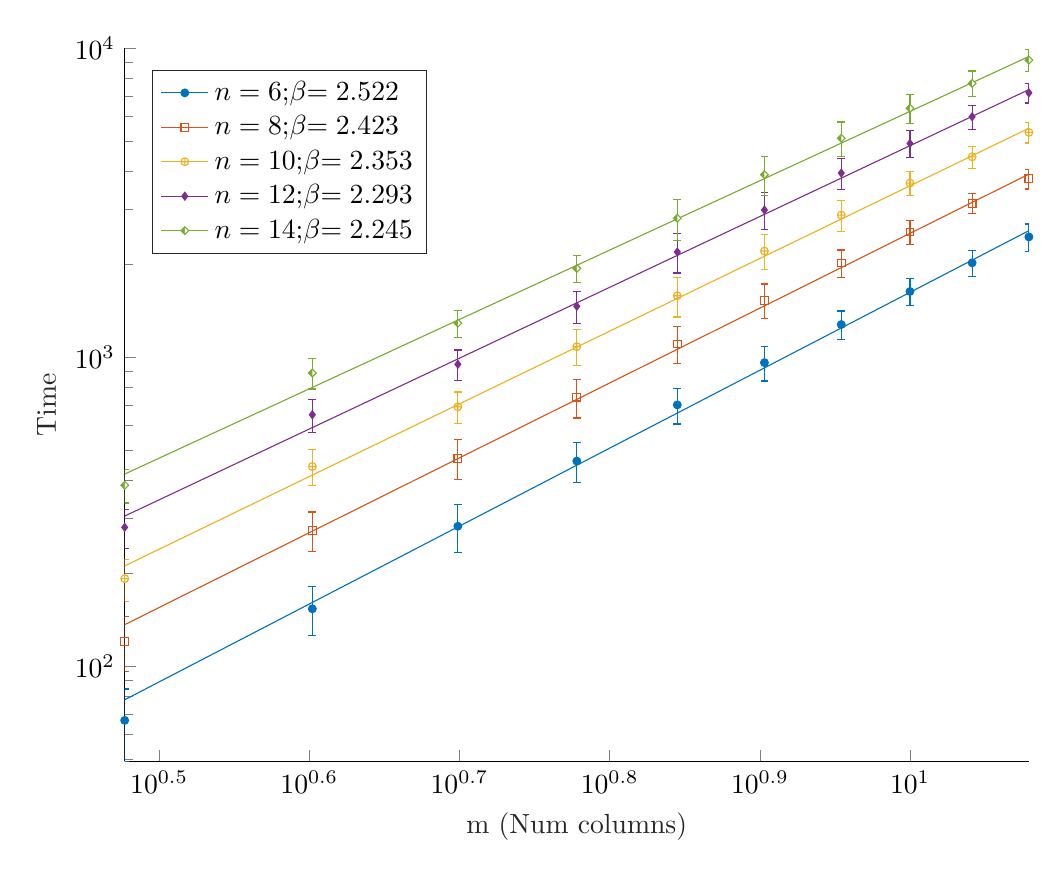
\begin{tikzpicture}

\begin{axis}[%
width=4.521in,
height=3.566in,
at={(0.758in,0.481in)},
scale only axis,
xmode=log,
xmin=3,
xmax=12,
xminorticks=true,
xlabel style={font=\color{white!15!black}},
xlabel={m (Num columns)},
ymode=log,
ymin=49.107205316463,
ymax=10000,
yminorticks=true,
ylabel style={font=\color{white!15!black}},
ylabel={Time},
axis background/.style={fill=white},
title style={font=\bfseries},
% title={$\text{Average ticks until solution as a function of m. On n }\times\text{ m grid. (k = 3)}$},
axis x line*=bottom,
axis y line*=left,
legend style={at={(0.03,0.97)}, anchor=north west, legend cell align=left, align=left, draw=white!15!black}
]
\addplot [color=mycolor1, draw=none, mark size=1.4pt, mark=*, mark options={solid, mycolor1}]
 plot [error bars/.cd, y dir = both, y explicit]
 table[row sep=crcr, y error plus index=2, y error minus index=3]{%
3	66.66	17.552794683537	17.552794683537\\
4	153.096	27.5215125184392	27.5215125184392\\
5	283.422	49.9995983551002	49.9995983551002\\
6	460.628	67.3539510752777	67.3539510752777\\
7	699.97	92.8015158426056	92.8015158426056\\
8	959.118	122.555701114846	122.555701114846\\
9	1274.124	135.21736610433	135.21736610433\\
10	1630.398	161.021811079389	161.021811079389\\
11	2018.254	192.250091493759	192.250091493759\\
12	2448.368	248.223751154628	248.223751154628\\
};
\addlegendentry{$\text{n =  6; }\beta\text{ = 2.522}$}

\addplot [color=mycolor1, forget plot]
  table[row sep=crcr]{%
3	77.7219683307341\\
4	160.577915617436\\
5	281.921996270413\\
6	446.532994420772\\
7	658.746455525474\\
8	922.562037973319\\
9	1241.71318540101\\
10	1619.71545357696\\
11	2059.90169007427\\
12	2565.44860338456\\
};
\addplot [color=mycolor2, draw=none, mark size=1.4pt, mark=square, mark options={solid, mycolor2}]
 plot [error bars/.cd, y dir = both, y explicit]
 table[row sep=crcr, y error plus index=2, y error minus index=3]{%
3	120.096	24.0455226251507	24.0455226251507\\
4	274.826	40.1585500520695	40.1585500520695\\
5	470.188	69.894399705702	69.894399705702\\
6	741.584	106.379340438566	106.379340438566\\
7	1102.424	149.829670239804	149.829670239804\\
8	1527.888	196.22465616577	196.22465616577\\
9	2015.708	205.586708045657	205.586708045657\\
10	2540.05	230.666646274243	230.666646274243\\
11	3146.168	236.087454873607	236.087454873607\\
12	3780.586	279.825014395359	279.825014395359\\
};
\addlegendentry{$\text{n =  8; }\beta\text{ = 2.423}$}

\addplot [color=mycolor2, forget plot]
  table[row sep=crcr]{%
3	136.054141022307\\
4	273.137803408996\\
5	468.976348202267\\
6	729.409281455014\\
7	1059.62714617573\\
8	1464.33800122329\\
9	1947.87353940914\\
10	2514.26159168155\\
11	3167.27822381892\\
12	3910.48663329908\\
};
\addplot [color=mycolor3, draw=none, mark size=1.4pt, mark=oplus, mark options={solid, mycolor3}]
 plot [error bars/.cd, y dir = both, y explicit]
 table[row sep=crcr, y error plus index=2, y error minus index=3]{%
3	191.742	29.9061899344063	29.9061899344063\\
4	442.14	59.2393704052636	59.2393704052636\\
5	690.392	80.7383161044046	80.7383161044046\\
6	1080.424	143.990161320537	143.990161320537\\
7	1579.256	231.641062049142	231.641062049142\\
8	2203.72	288.985693524998	288.985693524998\\
9	2882.014	339.238729562635	339.238729562635\\
10	3657.694	331.591897876705	331.591897876705\\
11	4447.706	371.577759866296	371.577759866296\\
12	5338.234	405.200644580851	405.200644580851\\
};
\addlegendentry{$\text{n = 10; }\beta\text{ = 2.353}$}

\addplot [color=mycolor3, forget plot]
  table[row sep=crcr]{%
3	210.833818153191\\
4	414.889543171822\\
5	701.407761631694\\
6	1077.18734831777\\
7	1548.18598379483\\
8	2119.74421735937\\
9	2796.7265082295\\
10	3583.61658229121\\
11	4484.58533033721\\
12	5503.54109952497\\
};
\addplot [color=mycolor4, draw=none, mark size=1.4pt, mark=diamond*, mark options={solid, mycolor4}]
 plot [error bars/.cd, y dir = both, y explicit]
 table[row sep=crcr, y error plus index=2, y error minus index=3]{%
3	281.08	40.6564569901262	40.6564569901262\\
4	650.48	79.0481804323118	79.0481804323118\\
5	947.736	106.761333208878	106.761333208878\\
6	1460.034	171.76972527498	171.76972527498\\
7	2188.854	316.965428477144	316.965428477144\\
8	2992.5	407.317238360139	407.317238360139\\
9	3942.424	456.829441368441	456.829441368441\\
10	4915.346	499.227758637266	499.227758637266\\
11	5997.69	530.711880496565	530.711880496565\\
12	7168.05	521.92107710021	521.92107710021\\
};
\addlegendentry{$\text{n = 12; }\beta\text{ = 2.293}$}

\addplot [color=mycolor4, forget plot]
  table[row sep=crcr]{%
3	305.62910181267\\
4	591.157835891336\\
5	986.136193717995\\
6	1498.01046464685\\
7	2133.22573892753\\
8	2897.5009878673\\
9	3796.0003504106\\
10	4833.44789156244\\
11	6014.20867811213\\
12	7342.34841800806\\
};
\addplot [color=mycolor5, draw=none, mark size=1.4pt, mark=halfsquare left*, mark options={solid, mycolor5}]
 plot [error bars/.cd, y dir = both, y explicit]
 table[row sep=crcr, y error plus index=2, y error minus index=3]{%
3	384.678	47.7708532983209	47.7708532983209\\
4	887.814	99.6067186529182	99.6067186529182\\
5	1287.79	128.313282621068	128.313282621068\\
6	1936.76	194.399776095272	194.399776095272\\
7	2815.5	429.856743159019	429.856743159019\\
8	3893.6	558.390702244141	558.390702244141\\
9	5105.982	660.682110684675	660.682110684675\\
10	6392.258	686.667593675724	686.667593675724\\
11	7692.926	739.409527544003	739.409527544003\\
12	9147.614	759.758951465967	759.758951465967\\
};
\addlegendentry{$\text{n = 14; }\beta\text{ = 2.245}$}

\addplot [color=mycolor5, forget plot]
  table[row sep=crcr]{%
3	418.043154280123\\
4	797.534519998318\\
5	1316.26763107558\\
6	1982.12950446365\\
7	2801.87973455616\\
8	3781.46774258057\\
9	4926.22861324372\\
10	6241.01335140422\\
11	7730.28033264396\\
12	9398.16220464329\\
};
\end{axis}
\end{tikzpicture}%
